\section{Experiments and Results}
\label{sec:experiments}

We evaluate our proposed consistency loss function on different datasets and using a variety of \gls{vqa} models.

\subsection{Datasets}
\label{subsec:cons_logic_datasets}

\subsubsection{Introspect~\cite{selvaraju2020squinting} } Contains perception questions (or sub-questions) created by annotators for a subset of reasoning questions (or main questions) of the \gls{vqa} v1.0 and v2.0 datasets~\cite{antol2015vqa,goyal2017making}. It contains 27,441 reasoning questions with 79,905 sub-questions in its training set and 15,448 reasoning questions with 52,573 sub-questions for validation. For images that have the same sub-question repeated multiple times, we remove duplicates in the sub-questions for every image in both the train and validation sets.

\subsubsection{DME Dataset~\cite{tascon2022consistency}} Consists of retinal fundus images for the task of \gls{dme} staging. It contains 9,779 QA pairs for training, 2,380 QA pairs for validation and 1,311 QA pairs for testing. There are three types of questions in the dataset: main, sub, and independent questions. Main questions ask about diagnosis information (\ie the stage of the disease) and sub-questions ask about the presence and location of biomarkers. Sub-questions are further subdivided into grade questions, questions about the whole image, questions about a region of the eye called macula, and questions about random regions in the image. To enable questions about image regions, we follow the procedure described in~\cite{tascon2022consistency}, whereby only the relevant region is shown to the model.


%%%%%%%%%%%%%%%%%%%%%%%%%%%%%%%

\subsection{Baseline Methods and Base Models} We consider 3 different consistency enhancement baseline methods. To ensure fair comparisons, all methods use the same \gls{vqa} base models and only differ in the consistency method used. These consist in:\\

{\setlength{\parindent}{0pt}\textit{- None:} Indicating that no consistency preserving method is used with the \gls{vqa} model. This corresponds to the case where $\lambda=0$.}

{\setlength{\parindent}{0pt}\textit{- SQuINT~\cite{selvaraju2020squinting}:} Optimizes consistency by maximizing the similarity between the attention maps of pairs of questions. As such, it requires a \gls{vqa} model that uses guided attention.}

{\setlength{\parindent}{0pt}\textit{- CP-VQA~\cite{tascon2022consistency}:} Assumes entailment relations and uses a regularizer to improve consistency.}


%(1) The case in which no consistency method is used, which corresponds to the case in which $\lambda=0$ in \ref{eq:total_loss}. So that the comparison is fair, for this baseline we also apply the pair sampling method described in \ref{sec:method} (\ie related pairs are in the same mini-batch). 
%(2) SQuINT~\cite{selvaraju2020squinting}, which is a method that aims at optimizing consistency by maximizing the similarity between the attention maps of pairs of questions. (3) Consistency-preserving VQA (C.P. VQA)~\cite{tascon2022consistency}, which assumes entailment relations and uses a regularizer to improve consistency. 

\subsubsection{VQA Architectures} We show experiments using three \gls{vqa} models depending on the dataset used. For experiments on Introspect, we make use of the \gls{ban} model~\cite{kim2018bilinear}, as its structure with guided attention allows the use of SQuINT. In addition, we evaluate the vision-language architecture LXMERT~\cite{tan2019lxmert} on this dataset to evaluate improvement in state-of-the-art, transformer-based \gls{vqa} models. For experiments on the \gls{dme} dataset, we use the base model described in~\cite{tascon2022consistency}, which we denote by MVQA. 


\subsection{Implementation Details}
\label{subsec:imp_details}
\subsubsection{LI-Model} We first pre-train \gls{bert} on SNLI for 5 epochs until it reaches a maximum accuracy of 84.32\% on that dataset. For this pre-training stage, we initialize \gls{bert} with the \textit{bert-base-uncased} weights and use a batch size of~16. We use a weight decay rate of 0.01 and the AdamW optimizer with a learning rate of $2\cdot10^{-5}$. The same setup was kept to finetune the model on a subset of 2'000 pairs of propositions from Introspect which were manually annotated (distribution of labels being: $\leftarrow 60\%, \leftrightarrow 17\%, - 12\%, \rightarrow  11\%$), and an additional 500 pairs were annotated for validation. Notice that LI-MOD is only necessary for the Introspect dataset since, for the \gls{dme} dataset, the implications annotations are available.

\subsubsection{VQA Models}
For our base models, we use the official and publicly available implementations (\gls{ban}~\cite{jackroos2019}, LXMERT~\cite{tan2019lxmert} and MVQA~\cite{tascon2022consistency}) with default configurations. We re-implemented SQuINT~\cite{selvaraju2020squinting} and used the provided implementation of CP-VQA~\cite{tascon2022consistency}, reporting the best results, which were obtained with $\lambda=0.1, \gamma=0.5$ for \gls{ban} and $\lambda=0.5, \gamma=1$ for MVQA (parameters refer to original implementations). For SQuINT, we set the gain of the attention map similarity term to 0.5 for \gls{ban} and 1.0 for MVQA. For Introspect, we train 5 models with different seeds for each parameter set and for \gls{dme}, we train 10 models with different seeds. To train LXMERT, \gls{ban} and MVQA, we use batch sizes of 32, 64 and 128, respectively. Regarding the \gls{vqa} cross-entropy loss, we follow the original implementations and use soft scores for the answers in LXMERT and categorical answers for \gls{ban} and MVQA.

%%%---------------------------%%%
\subsection{Quantifying Consistency}
%$Given a test set, $\mathcal{T}= \{t_n\}^{=1,\ldots,|\mathcal{T}|}$, where $t_n=(\x, \q, a) $ is a test sample triplet, we evaluate the performance of all models using the strict accuracy of predictions as in ~\cite{selvaraju2020squinting,vu2020question} by computing,
%\begin{equation}
%    acc = \frac{1}{|\mathcal{T}|}\sum_{n=1}^{|\mathcal{T}|} 1_{ \{a^n = \tilde{a}^n \}},
%\end{equation}
%where $\tilde{a}^n = \argmax_{a^* \in \mathcal{A}} p(a^* | \x^n,\q^n; \theta)$ is the produced answer of an evaluated method. \STM{I think we could omit the definition of accuracy here. Most recent CVPR papers on consistency only mention that they use accuracy. This would be easier because LXMERT computes the accuracy slightly differenttly due to the soft scores of the GT answers}

Given a test set~$\mathcal{T}= \{t_n\}_{n=1}^{|\mathcal{T}|}$, where $t_n=(\x, \q, a)$ is a test sample triplet, we wish to measure the level of consistency of a \gls{vqa} model~$p$. To this end, we define the set of implications~$G(\mathcal{T}) \subset \mathcal{T}^2$ as the collection of all pairs of test samples~$((\x_i, \q_i, a_i), (\x_j, \q_j, a_j))$ for which~$(\q_i, a_i) \rightarrow (\q_j, a_j)$ and~$\x_i=\x_j$,
% To do so, we define $G_\leftarrow$, $G_\rightarrow$, $G_\leftrightarrow$, $G_\leftrightarrow$ and $G_{-}$ as sets containing all image-question-answer triplets in $\mathcal{T}$ according to their relation. For instance, $G_\leftarrow$ contains all pairs $((\x, \q_i, a_i), (\x, \q_j, a_j))$ for which $(\q_i, a_i) \leftarrow (\q_j, a_j)$. 
and the set of inconsistencies~$I_p(\mathcal{T})$ produced by the \gls{vqa} model as the subset of~$G(\mathcal{T})$ that contains the pairs for which the model evaluated the sufficient condition as true and the necessary condition as false,
\begin{equation}
    \nonumber
    I_p(\mathcal{T}) = \{ (t_i, t_j)\in G(\mathcal{T})\mid
     e_p((\q_i, a_i), \x) \wedge \neg e_p((\q_j, a_j), \x)\}.
\end{equation}
% We count the inconsistencies produced by a VQA model~$p$ evaluated on~$\mathcal{T}$ as the number of times the model evaluates a sufficient condition as true and a necessary condition as false,
% \begin{equation}
%     I_p(\mathcal{T}) = \sum_{(t_i, t_j)\in G(\mathcal{T})} \mathbbm{1}[e_p((\q_i, a_i), \x) \wedge \neg e_p((\q_j, a_j), \x)].
% \end{equation}
The function~$e_p$ returns the truth value of the proposition~$(\q, a)$ for image~$\x$ evaluated by the \gls{vqa} model~$p$,
\begin{equation}
    e_p((\q, a), \x) = [\hat{a}=a],
\end{equation}
where $\hat{a}$ is the answer of maximum probability following Eq.~\eqref{eq:vqa}. In other words, $e_p$~returns whether the estimated answer for question~$\q$ matches the answer of the proposition~$a$.
Finally, the consistency ratio~$c$ for model~$p$ on the test set~$\mathcal{T}$ is the proportion of implications in~$G(\mathcal{T})$ that did not lead to an inconsistency,
\begin{equation}
    c_p(\mathcal{T}) = 1 - \dfrac{|I_p(\mathcal{T})|}{|G(\mathcal{T})|}.
\end{equation}
% \begin{equation}
%     c() = 1 - \frac{I_{\rightarrow} + I_{\leftarrow} + I_{\leftrightarrow}}{|G_{\leftarrow}| + |G_{\leftarrow}| + 2|G_{\leftrightarrow}|}.
%     \label{eq:consistency_metric}
% \end{equation}


% REsults
\subsection{Results}
\label{sec:cons_logic_results}

%%%---------------------------%%%
%%%---------------------------%%%

\subsubsection{Performance Comparison}
For both datasets, we first compare the performance of our method against the baseline consistency methods in Tables \ref{tab:results_introspect} and \ref{tab:cons_logic_results_dme}. In either case, we see that our method outperforms previous approaches by not only increasing overall prediction accuracy but also by increasing consistency. In Figures \ref{fig:examples_introspect} and \ref{fig:examples_dme}, we show illustrative examples of our approach on the Introspect and \gls{dme} datasets, respectively (see additional examples in Appendix~\ref{appendix:consistency_logic}).

%\begin{table}[!b ]
%  \centering
%  \begin{tabular}{@{}lccc@{}}
%    \toprule
%     Model & Cons. Method & Acc. & Cons. \\
%     \midrule
%     BAN & None & 67.14$\pm$0.10 & 69.45$\pm$0.17 \\
%     BAN & SQuINT~\cite{selvaraju2020squinting} & 67.27$\pm$0.19 & 69.87$\pm$0.45 \\
%     BAN & CP-VQA~\cite{tascon2022consistency} & 67.18$\pm$0.24 & 69.52$\pm$0.45\\
%     BAN & {\bf Ours} ($\lambda=0.01$) & {\bf 67.36$\pm$0.19} & {70.38$\pm$0.39} \\
%    \midrule
%    LXMERT & None & 75.10$\pm$0.10 & 76.24$\pm$0.63 \\
%    LXMERT & Random flip & 69.67$\pm$1.24 & 75.99$\pm$3.91\\
%    LXMERT & Flip first & 73.81$\pm$0.47 & 71.94$\pm$2.82\\
%    LXMERT & Flip second & 65.82$\pm$1.03 & {87.56$\pm$2.51}\\
%    LXMERT & {\bf Ours} & {\bf 75.17$\pm$0.08} & {78.75$\pm$0.21} \\
%    \bottomrule
%  \end{tabular}
%  \caption{Results of different consistency methods on the Introspect dataset using two different VQA models: (top) BAN and (bottom) LXMERT. In the case of LXMERT, we show the impact of randomly flipping the answer of either the first or the second question for pairs detected as inconsistent using the relations from LI-MOD. Similarly, {\it flip first} and {\it flip second} refer to flipping the answer of the first and second question in inconsistent pairs, respectively. \STM{STDs added}}
%  \label{tab:results_introspect}
%\end{table}


\begin{table}[!b ]
  \centering
  \begin{tabular}{@{}llcc@{}}
    \toprule
     Model & Cons. Method & Acc. & Cons. \\
     \midrule
     \multirow{4}{*}{BAN} & None & 67.14$\pm$0.10 & 69.45$\pm$0.17 \\
      & SQuINT~\cite{selvaraju2020squinting} & 67.27$\pm$0.19 & 69.87$\pm$0.45 \\
      & CP-VQA~\cite{tascon2022consistency} & 67.18$\pm$0.24 & 69.52$\pm$0.45\\
      & {\bf Ours} ($\lambda=0.01$) & {\bf 67.36$\pm$0.19} & {70.38$\pm$0.39} \\
    \midrule
    \multirow{5}{*}{LXMERT} & None & 75.10$\pm$0.10 & 76.24$\pm$0.63 \\
     & Random flip & 69.67$\pm$1.24 & 75.99$\pm$3.91\\
     & Flip first & 73.81$\pm$0.47 & 71.94$\pm$2.82\\
     & Flip second & 65.82$\pm$1.03 & {87.56$\pm$2.51}\\
     & {\bf Ours} & {\bf 75.17$\pm$0.08} & {78.75$\pm$0.21} \\
    \bottomrule
  \end{tabular}
  \caption{Results of different consistency methods on the Introspect dataset using two different VQA models: \textbf{Top:} BAN, \textbf{bottom:} LXMERT. In the case of LXMERT, we show the impact of randomly flipping the answer of either the first or the second question for related pairs. Similarly, {\it flip first} and {\it flip second} refer to flipping the answer to the first and second question in inconsistent pairs, respectively.}
  \label{tab:results_introspect}
\end{table}

\begin{table*}[t]
\centering
\begin{tabular}{@{}llcccccr@{}}
\toprule
\multirow{2}{*}{Model} &  \multicolumn{1}{l}{\multirow{2}{*}{Consis. Method}}   & \multicolumn{5}{c}{Accuracy}  & \multicolumn{1}{c}{\multirow{2}{*}{Consistency}} \\ \cline{3-7}
\multicolumn{1}{c}{}         &\multicolumn{1}{c}{}                  & \multicolumn{1}{c}{all} & \multicolumn{1}{l}{grade} & \multicolumn{1}{c}{whole} & \multicolumn{1}{c}{macula} & \multicolumn{1}{c}{region} & \multicolumn{1}{l}{}                             \\ 
\midrule
\multirow{4}{*}{MVQA}     &   \multicolumn{1}{l}{None}          & \multicolumn{1}{c}{81.15$\pm$0.49}   & \multicolumn{1}{c}{78.17$\pm$2.07} & \multicolumn{1}{c}{83.44$\pm$1.87} & \multicolumn{1}{c}{87.25$\pm$1.20}  & \multicolumn{1}{c}{80.38$\pm$2.02}  & \multicolumn{1}{c}{89.95$\pm$3.20}                        \\ 

 &  \multicolumn{1}{l}{SQuINT~\cite{selvaraju2020squinting}}& \multicolumn{1}{c}{80.58$\pm$0.78}   & \multicolumn{1}{c}{77.48$\pm$0.40} & \multicolumn{1}{c}{82.82$\pm$0.74} & \multicolumn{1}{c}{85.34$\pm$0.87}  & \multicolumn{1}{c}{80.02$\pm$1.03}  & \multicolumn{1}{c}{89.39$\pm$2.12}               
\\ 

 &  \multicolumn{1}{l}{CP-VQA~\cite{tascon2022consistency}}& \multicolumn{1}{c}{83.49$\pm$0.99}   & \multicolumn{1}{c}{\textbf{80.69$\pm$1.30}} & \multicolumn{1}{c}{84.96$\pm$1.14} & \multicolumn{1}{c}{87.18$\pm$2.18} & \multicolumn{1}{c}{\textbf{83.16$\pm$1.09}}  & \multicolumn{1}{c}{94.20$\pm$2.15}  
\\ 

 &  
\multicolumn{1}{l}{{\bf Ours} ($\lambda=0.25$)}& \multicolumn{1}{c}{\textbf{83.59$\pm$0.69}}   & \multicolumn{1}{c}{80.15$\pm$0.95} & \multicolumn{1}{c}{\textbf{86.22$\pm$1.67}} & \multicolumn{1}{c}{\textbf{88.18$\pm$1.07}}  & \multicolumn{1}{c}{82.62$\pm$1.02}  & \multicolumn{1}{c}{{95.78$\pm$1.19}}  

\\ \bottomrule
                                                 
\end{tabular}
\caption{Comparison of methods on the DME dataset with common MVQA backbone. Accuracy and consistency are reported for all questions, as well as for different medically relevant sub-question categories: grade, whole, macula and region.
}
\label{tab:cons_logic_results_dme}
\end{table*}
\begin{figure*}[!t]
\centering
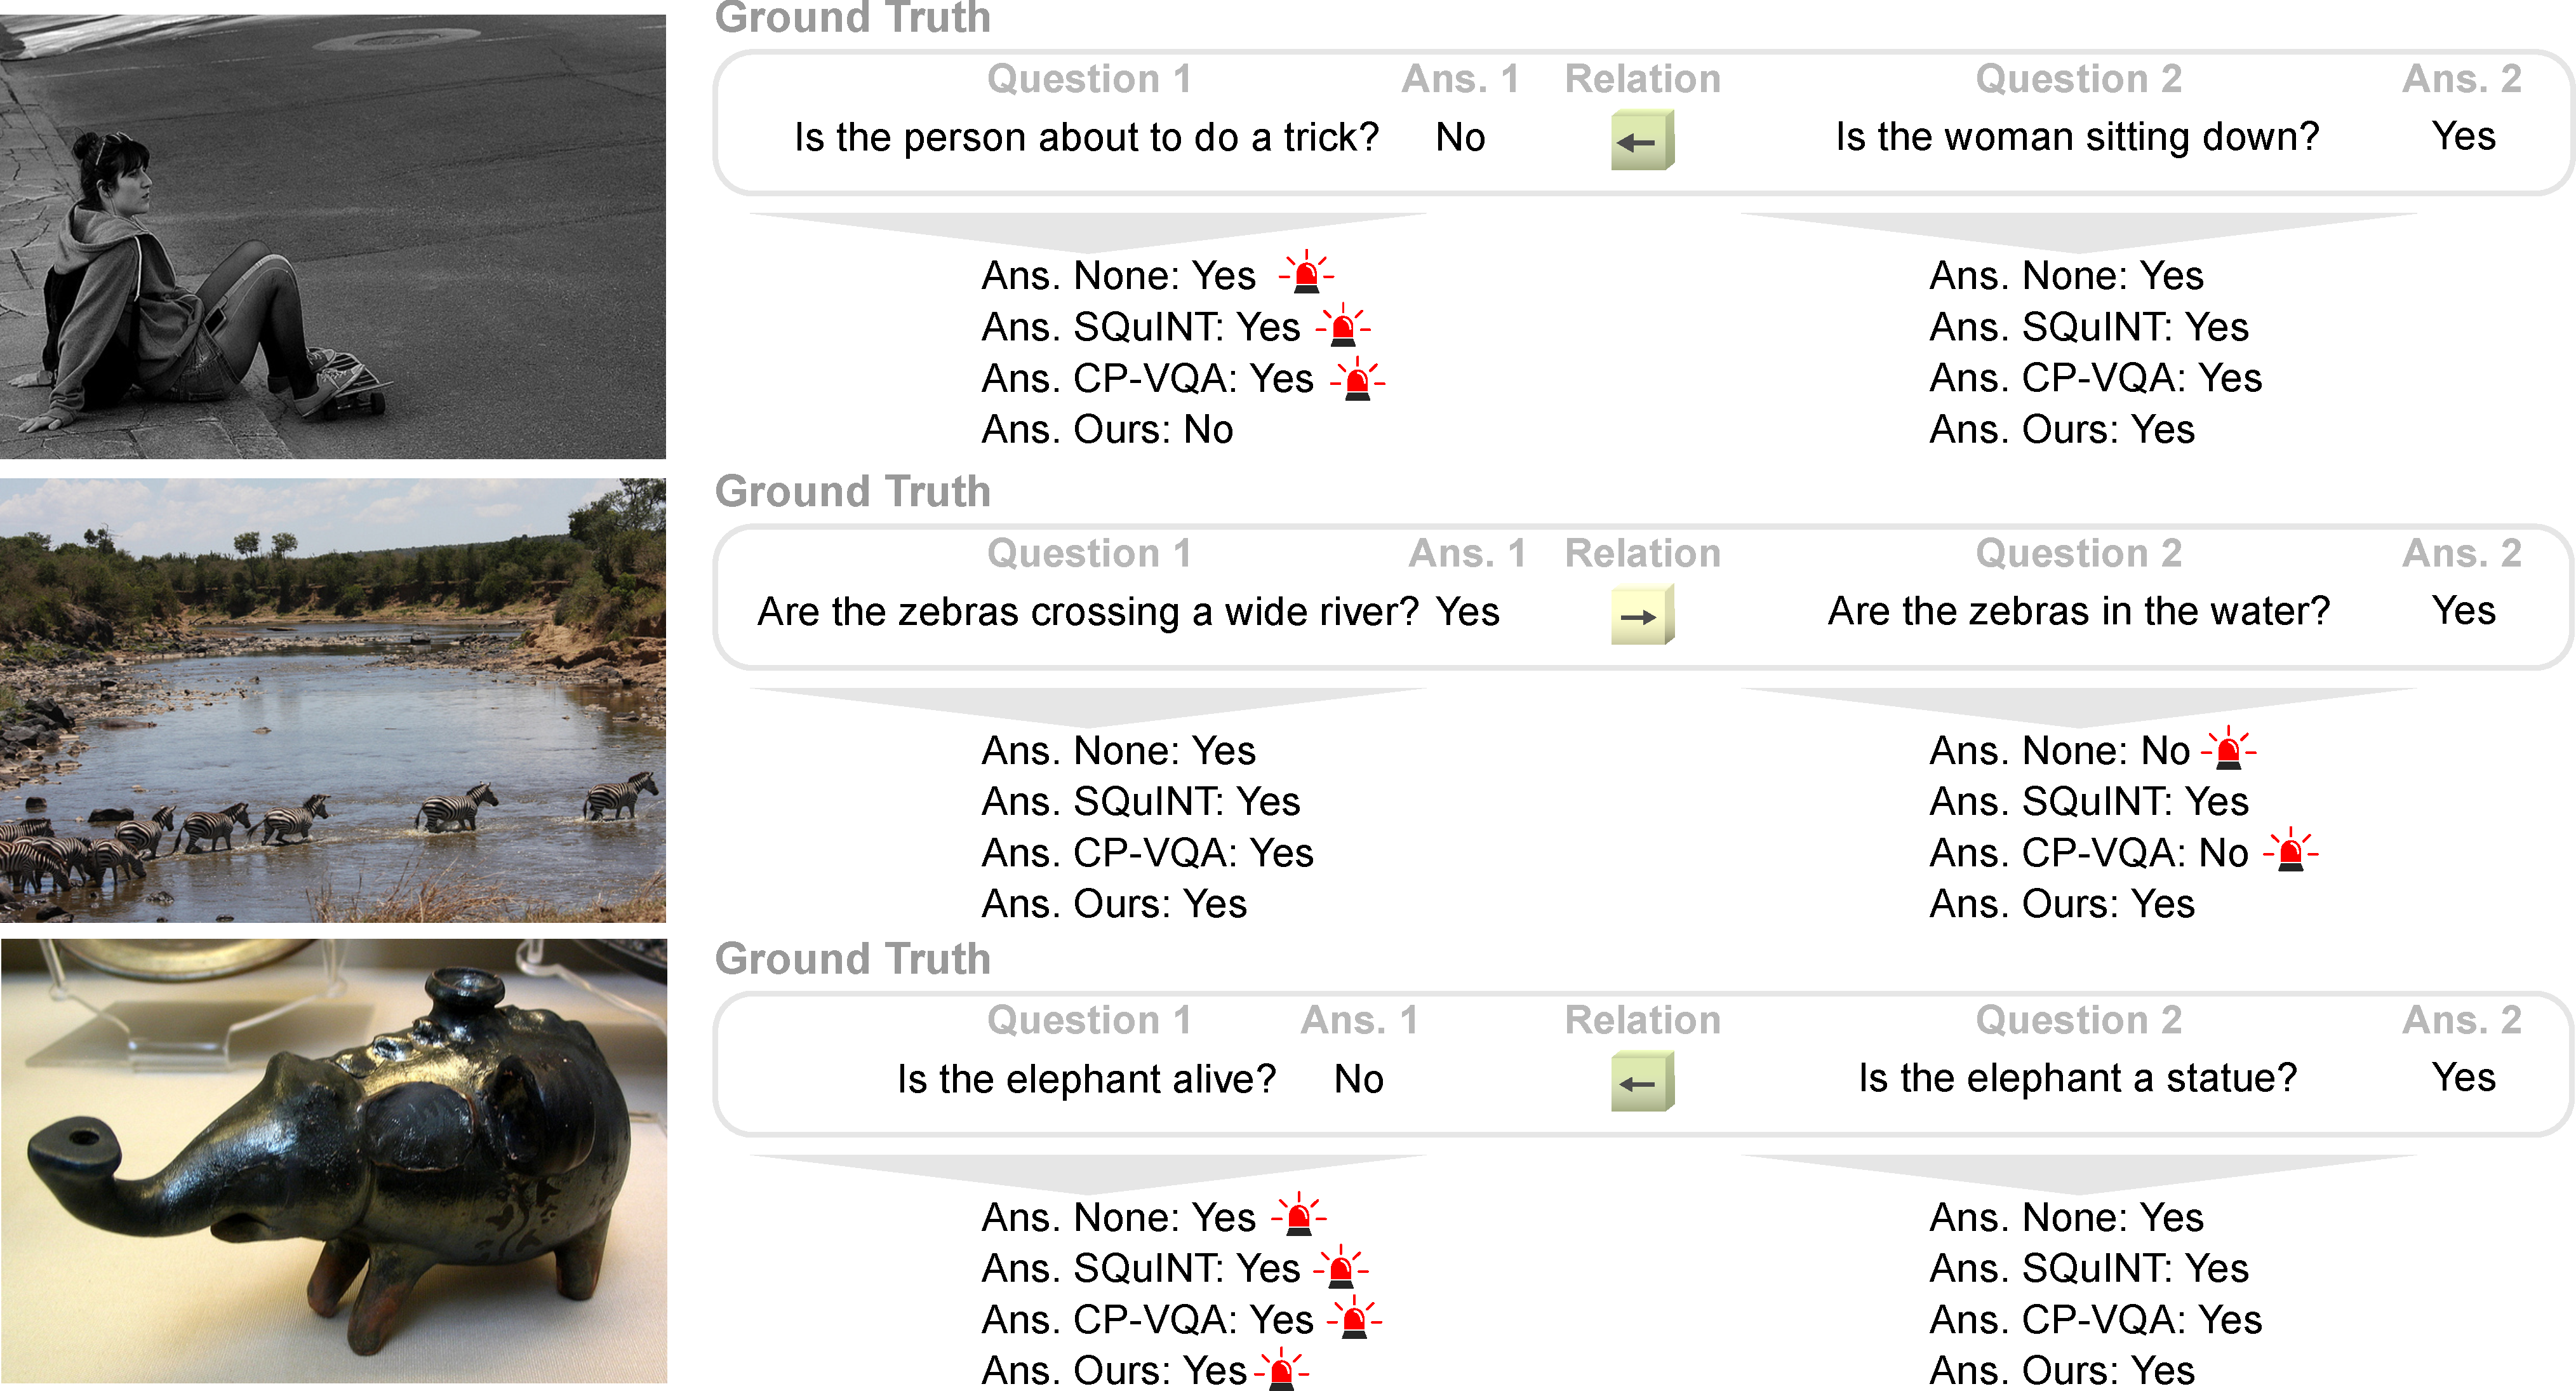
\includegraphics[width=0.95\textwidth]{Figures/Part2_Consist/02_logic/examples_ban.pdf}
\caption{Qualitative examples from the Introspect dataset using BAN as backbone. Red siren symbols indicate inconsistent cases.}
\label{fig:examples_introspect}
\end{figure*}
\begin{figure*}[!t]
\centering
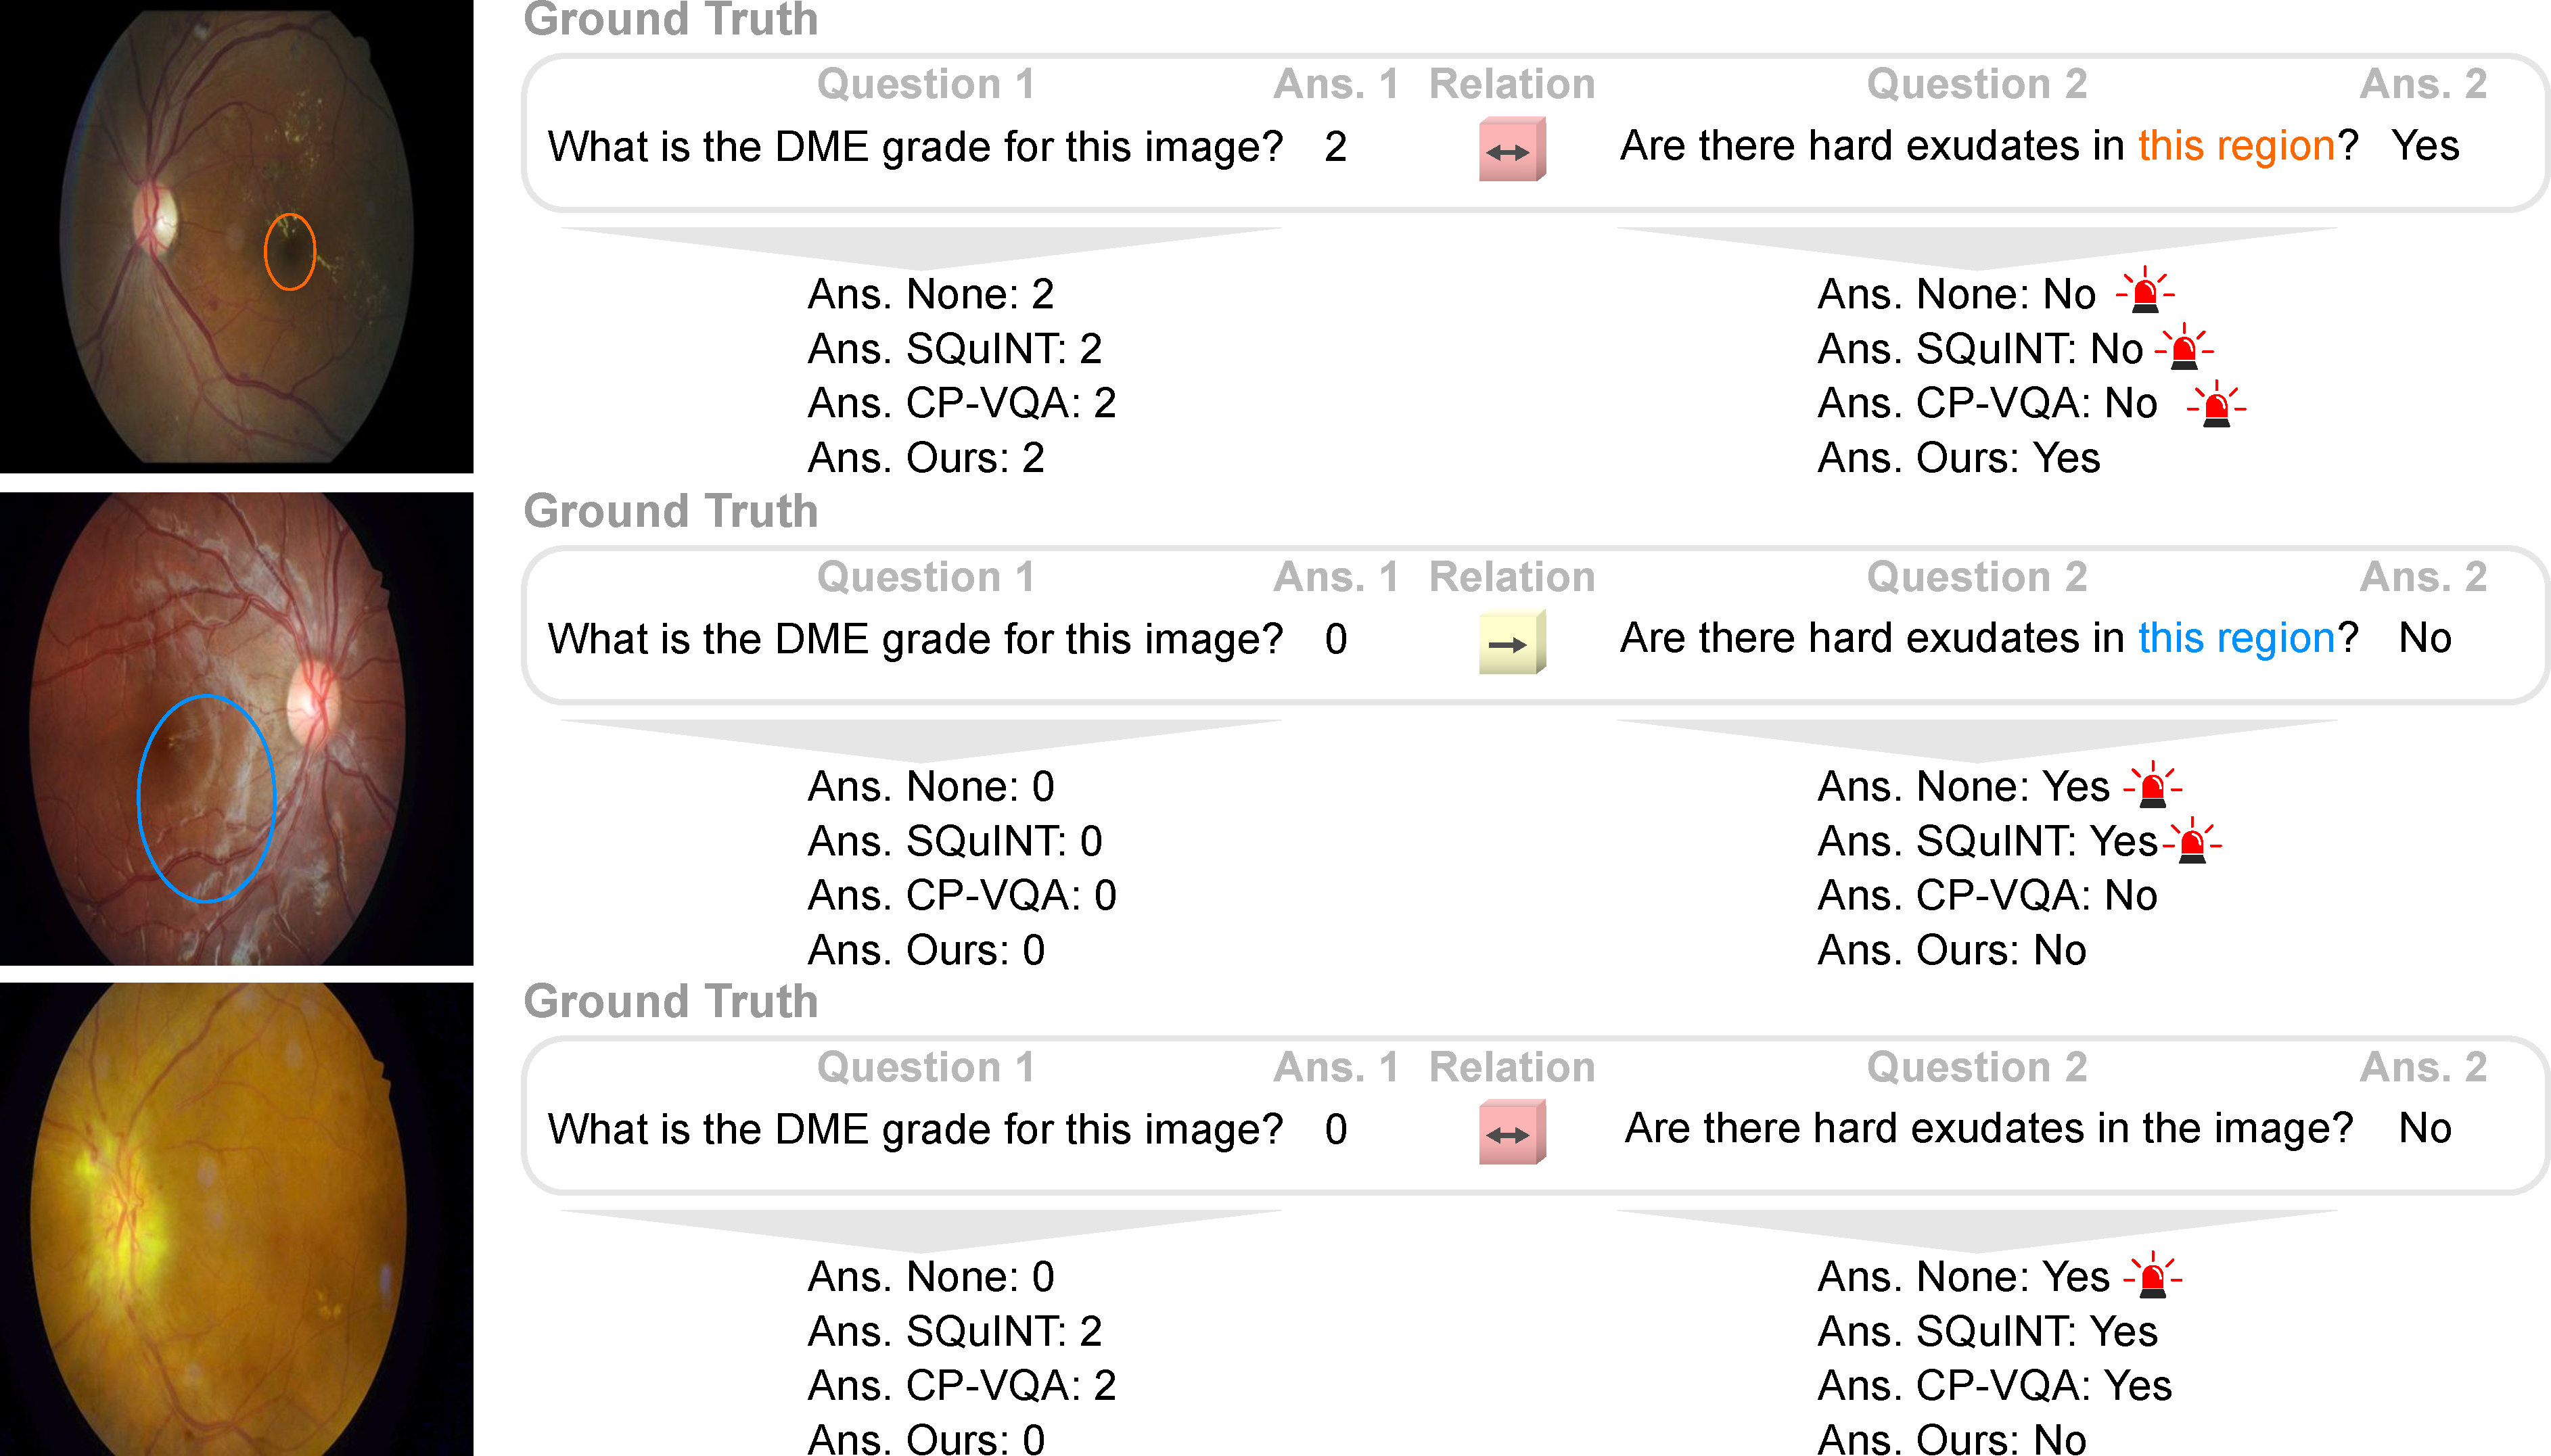
\includegraphics[width=0.90\textwidth]{Figures/Part2_Consist/02_logic/examples_dme.pdf}
\caption{Examples from the DME dataset and comparison of methods. Red siren symbols indicate inconsistent cases. DME is a disease that is staged into grades (0, 1 or 2), which depend on the number of visual pathological features of the retina. \textbf{Top} and \textbf{middle:} Although all methods correctly predict the answer to the first question, some inconsistencies appear when a necessary condition is false. \textbf{Bottom}: Only the None baseline produces an inconsistency. Note that SQuINT and CP-VQA's answers do not produce inconsistent pairs because both questions were answered incorrectly, and those answers (``2" and ``yes") respect all known relations. 
}
\label{fig:examples_dme}
\end{figure*} 

In Table \ref{tab:results_introspect}, we also show the performance of the state-of-the-art LXMERT \gls{vqa} model when combined with our method. In this case, too, we see that our method provides increased performance via consistency improvements. Here we investigate the performance induced when flipping the answers of one of the members of each related pair at test time. Suppose implication labels are present, either by manual annotation or by LI-MOD. In that case, a trivial manner of correcting an inconsistent QA pair of binary answers is to flip or negate one of the answers. This is far simpler than our proposed method as it permits training the \gls{vqa} model with the standard \gls{vqa} loss. Having obtained the answers from the model when $\lambda=0$, we identify the related pairs and then flip the answers (1) either randomly, (2) of the first QA or (3) of the second QA. By including the flipping baselines, we confirm that the added complexity in training our method results in improved accuracy compared to merely correcting inconsistencies post-hoc. Increases in consistency at the expense of accuracy are explained by the fact that an inconsistent QA pair guarantees that one of the two answers is incorrect, but correcting the inconsistency does not necessarily fix the incorrect answer. This phenomenon is particularly noticeable in the flipping baselines, as they fix inconsistencies without considering their correctness.

In general, we observe that training LXMERT with our consistency loss provides performance gains. Indeed, while random flipping based on LI-MOD clearly deteriorates the performance of LXMERT, so does flipping the first or second answers. This implies that our proposed method indeed leverages the predictions of LI-MOD to make LXMERT more consistent as it improves both model accuracy and consistency. 
\begin{figure}[!t]
\centering
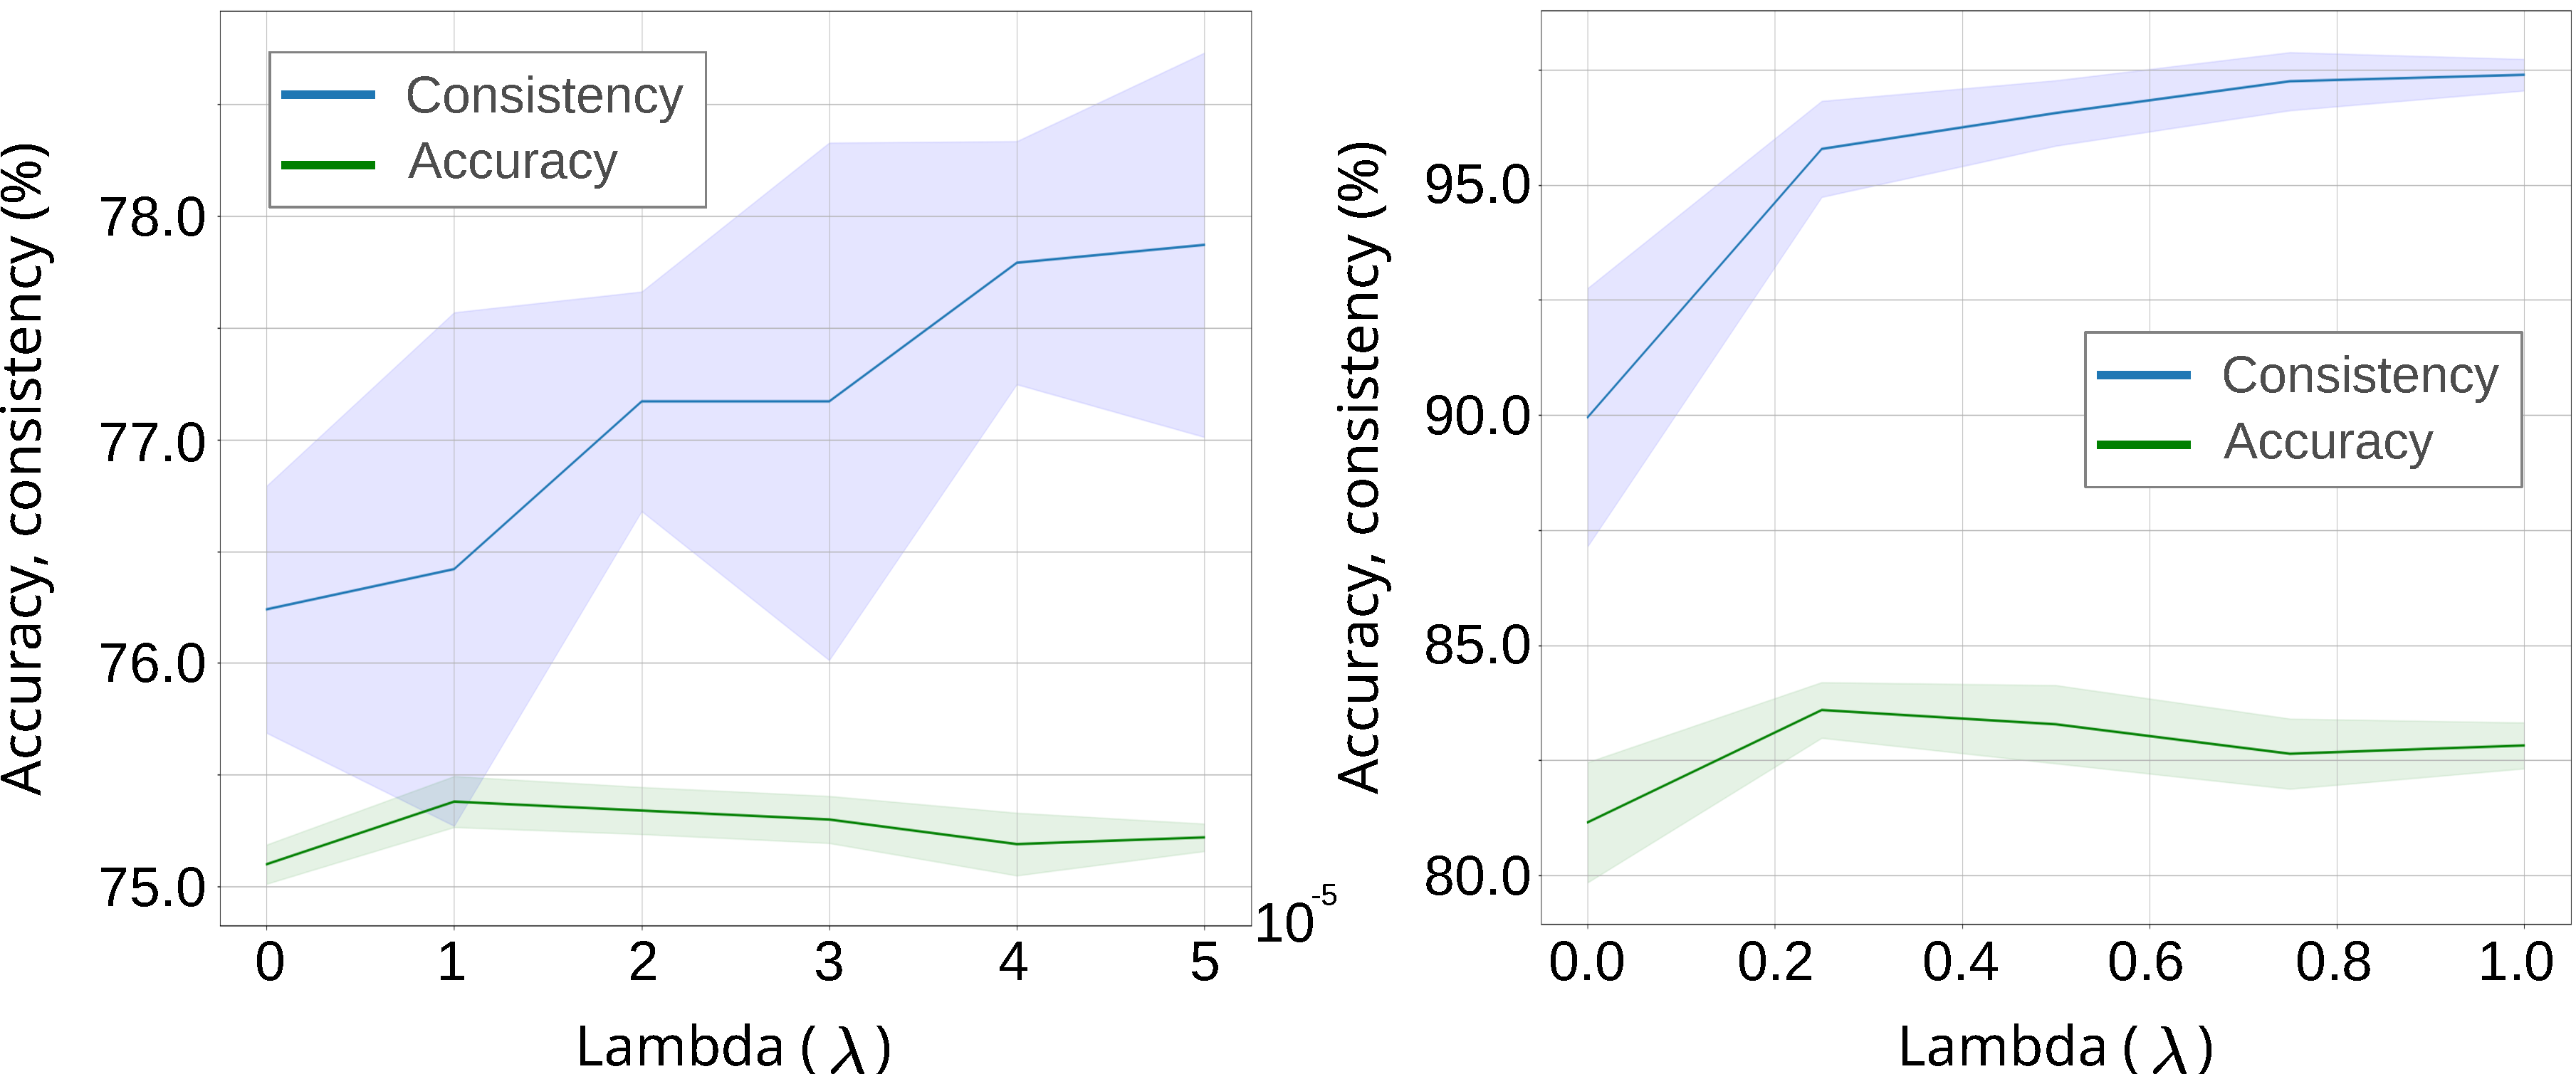
\includegraphics[width=0.8\textwidth]{Figures/Part2_Consist/02_logic/lambda_s.pdf}
\caption{Behavior of the accuracy and consistency as a function of $\lambda$ with 95\% confidence intervals. \textbf{Left:} LXMERT trained on the Introspect dataset (5 models with random seeds for each value of $\lambda$). \textbf{Right:} MVQA trained on the DME dataset (10 models with random seeds for each $\lambda$).}
\label{fig:lambda}
\end{figure}
\subsubsection{Sensitivity of $\bm{\lambda}$}  We now show the sensitivity of our method and its relation to $\lambda$. We evaluate the performance of our method for different values of $\lambda$ to understand the behavior of the performance, both in terms of accuracy and consistency. 

\fig~\ref{fig:lambda} shows the accuracy and consistency of LXMERT and MVQA for different values of $\lambda$. The difference in the ranges of the values is due to the relative magnitude of the loss function terms and depends on the used loss functions (\eg, binary and non-binary cross-entropy) and the ground-truth answer format (\ie, soft scores for LXMERT, as mentioned in Sec.~\ref{subsec:imp_details}). 

In general, we observe very similar behavior for the accuracy, which increases and then slowly decreases as $\lambda$ increases. We sustain that the maximum value the accuracy can reach is established by the number of related pairs that are still inconsistent after training with $\lambda=0$. In other words, the limitations in size impose a limit on how much our method can improve the accuracy. For LXMERT on Introspect, for instance, our model corrected 4,553 (78.9\%) of the 5’771 existing inconsistencies and introduced new inconsistencies by mistakenly altering 1,562 (3.5\%) of the 44,111 consistent samples.

Regarding consistency, we observe a constant increase as $\lambda$ increases. The simultaneous decrease in accuracy as $\lambda$ increases suggests that the relative weight of the consistency loss dominates so that the model no longer focuses on optimizing the cross-entropy. Since it is possible to be consistent without answering correctly, the optimization process results in an increase in consistency at the expense of accuracy for higher values of $\lambda$. However, it is clear from these results that there is a set of $\lambda$ values for which both metrics improve.


 

%\begin{table*}[!t]
%  \centering
%  \begin{tabular}{@{}lccr@{}}
%    \toprule
%    Model & Cons. Method & Acc. & Cons. \\
%    \midrule
%    Base & None & 81.15 & 89.95 \\
%    Base & SQuINT~\cite{selvaraju2020squinting} & 80.58 & 89.39 \\
%    Base & Ours & \textbf{82.85} & \textbf{95.09} \\
%    \bottomrule
%  \end{tabular}
%  \caption{Results on the DME dataset.}
%  \label{tab:cons_logic_results_dme}
%\end{table*}





%\begin{figure}[!t]
%\centering
%\includegraphics[width=0.45\textwidth]{images/dme_plot_consacc_vs_lambda.pdf}
%\caption{Behavior of the accuracy and consistency as a function of the loss term gain $\lambda$ for the DME dataset. 95\% confidence intervals are shown.}
%\label{fig:method}
%\end{figure}


\subsubsection{LI-MOD Performance} We report that the finetuning of \gls{bert} on the subset of annotated relations from Introspect produced $78.67\%$ accuracy in the \gls{nli} task. We analyze the performance of this model for entailment and report an AUC value of 0.86, which indicates good generalization capability considering that only $\approx 2 \%$ of the dataset was annotated with relations. In addition, the overlap in the QA pairs between the train and validation sets of the Introspect dataset is only 1.12\% for binary questions. This shows that our LI-MOD is generalizing to variations in questions and to new combinations of QA pairs. \fig~\ref{fig:roc_dot} shows the \gls{roc} curve for entailment and examples of LI-MOD's predictions. Some of the observed sources of errors in LI-MOD include negations, unusual situation descriptions (\eg, a cat typing a text message), and image-specific references (\eg, ``is \textit{this} animal real?"). 
\begin{figure}
    \centering
    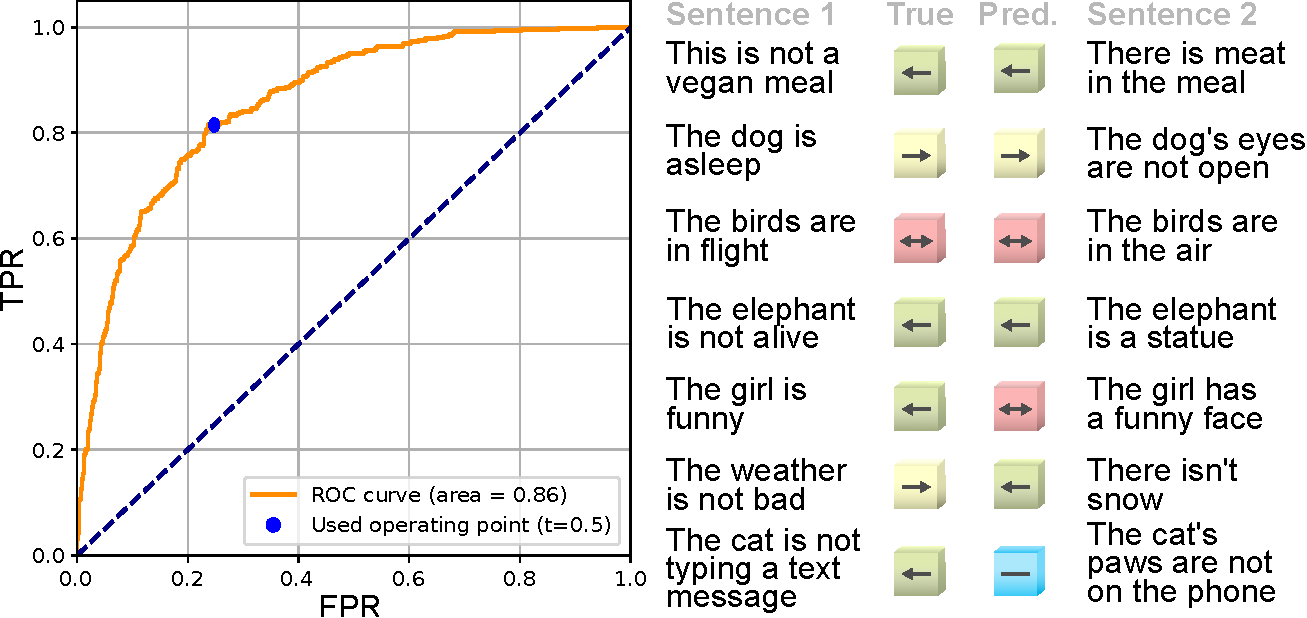
\includegraphics[width=0.8\linewidth]{Figures/Part2_Consist/02_logic/roc_examples_s.pdf}
    \caption{\textbf{Left:} Receiver Operating Characteristic (ROC) for the entailment class of our LI-MOD in validation. \textbf{Right:} Qualitative examples of LI-MOD's predictions.}
    \label{fig:roc_dot}
\end{figure}

%\begin{figure}[!t]
%\centering
%\includegraphics[width=0.4\textwidth]{images/roc.png}
%    \caption{Receiver Operating Characteristic (ROC) for the entailment class of our LI-MOD in validation}
%\label{fig:roc}
%\end{figure}

%\RS{What is the distribution of relations per group in the train and test sets you annotated?} \STM{For train it is $(\leftarrow : 0.595, \leftrightarrow: 0.1725, -: 0.1175, \rightarrow : 0.109, contradictions: 0.006)$. For val it's fairly similar: $(\leftarrow : 0.572, \leftrightarrow: 0.142, -: 0.156, \rightarrow : 0.109)$}

%\begin{figure}[!t]
%\centering
%\includegraphics[width=0.35\textwidth]{images/confusion_matrix_rels.pdf}
%\caption{Confusion matrix for logical implication prediction using our proposed LI-MOD strategy. Note that distribution of labels in both the training used to is given $(\leftarrow : 60\%, \leftrightarrow: 17\%, -: 12\%, \rightarrow : 11\%)$, while the validation set (performance shown here) follows a similar distribution.}
%\label{fig:confusion_matrix}
%\end{figure}